\documentclass{article}
\usepackage[margin=1.1in]{geometry}
\usepackage{undertilde, amsmath, amsfonts, commath, cancel, graphicx}
\usepackage{accents}

\newcommand{\ut}[1]{\underaccent{\tilde}{#1}}

\title{PHYS 7125 Homework 5}
\author{Wenqi He}
\begin{document}
\maketitle
\section{}
The total proper time along any curve $\gamma$ is
\begin{align*}
\tau_{total} &= \int_\gamma d\tau = \int_\gamma \sqrt{-ds^2} 
= \int_\gamma \sqrt{-\Big(\frac{2M}{r} - 1\Big)dt^2 + \Big(\frac{2M}{r} -1 \Big)^{-1} dr^2 - r^2d\Omega^2}
\end{align*}
Inside the event horizon, $r < 2M$, the first and third term in the square root are negative, therefore
\begin{align*}
\tau_{total} &< \int^{2M}_0 \sqrt{\Big(\frac{2M}{r} -1 \Big)^{-1}} dr \\
&= \Bigg[ -\sqrt{r(2M-r)} + 2M\cot^{-1}\left(\sqrt{\frac{2M}{r}-1} \right) \Bigg] \Bigg\rvert^{2M}_0 = \pi M
\end{align*}
\section{}
\subsection*{a}
\begin{center}
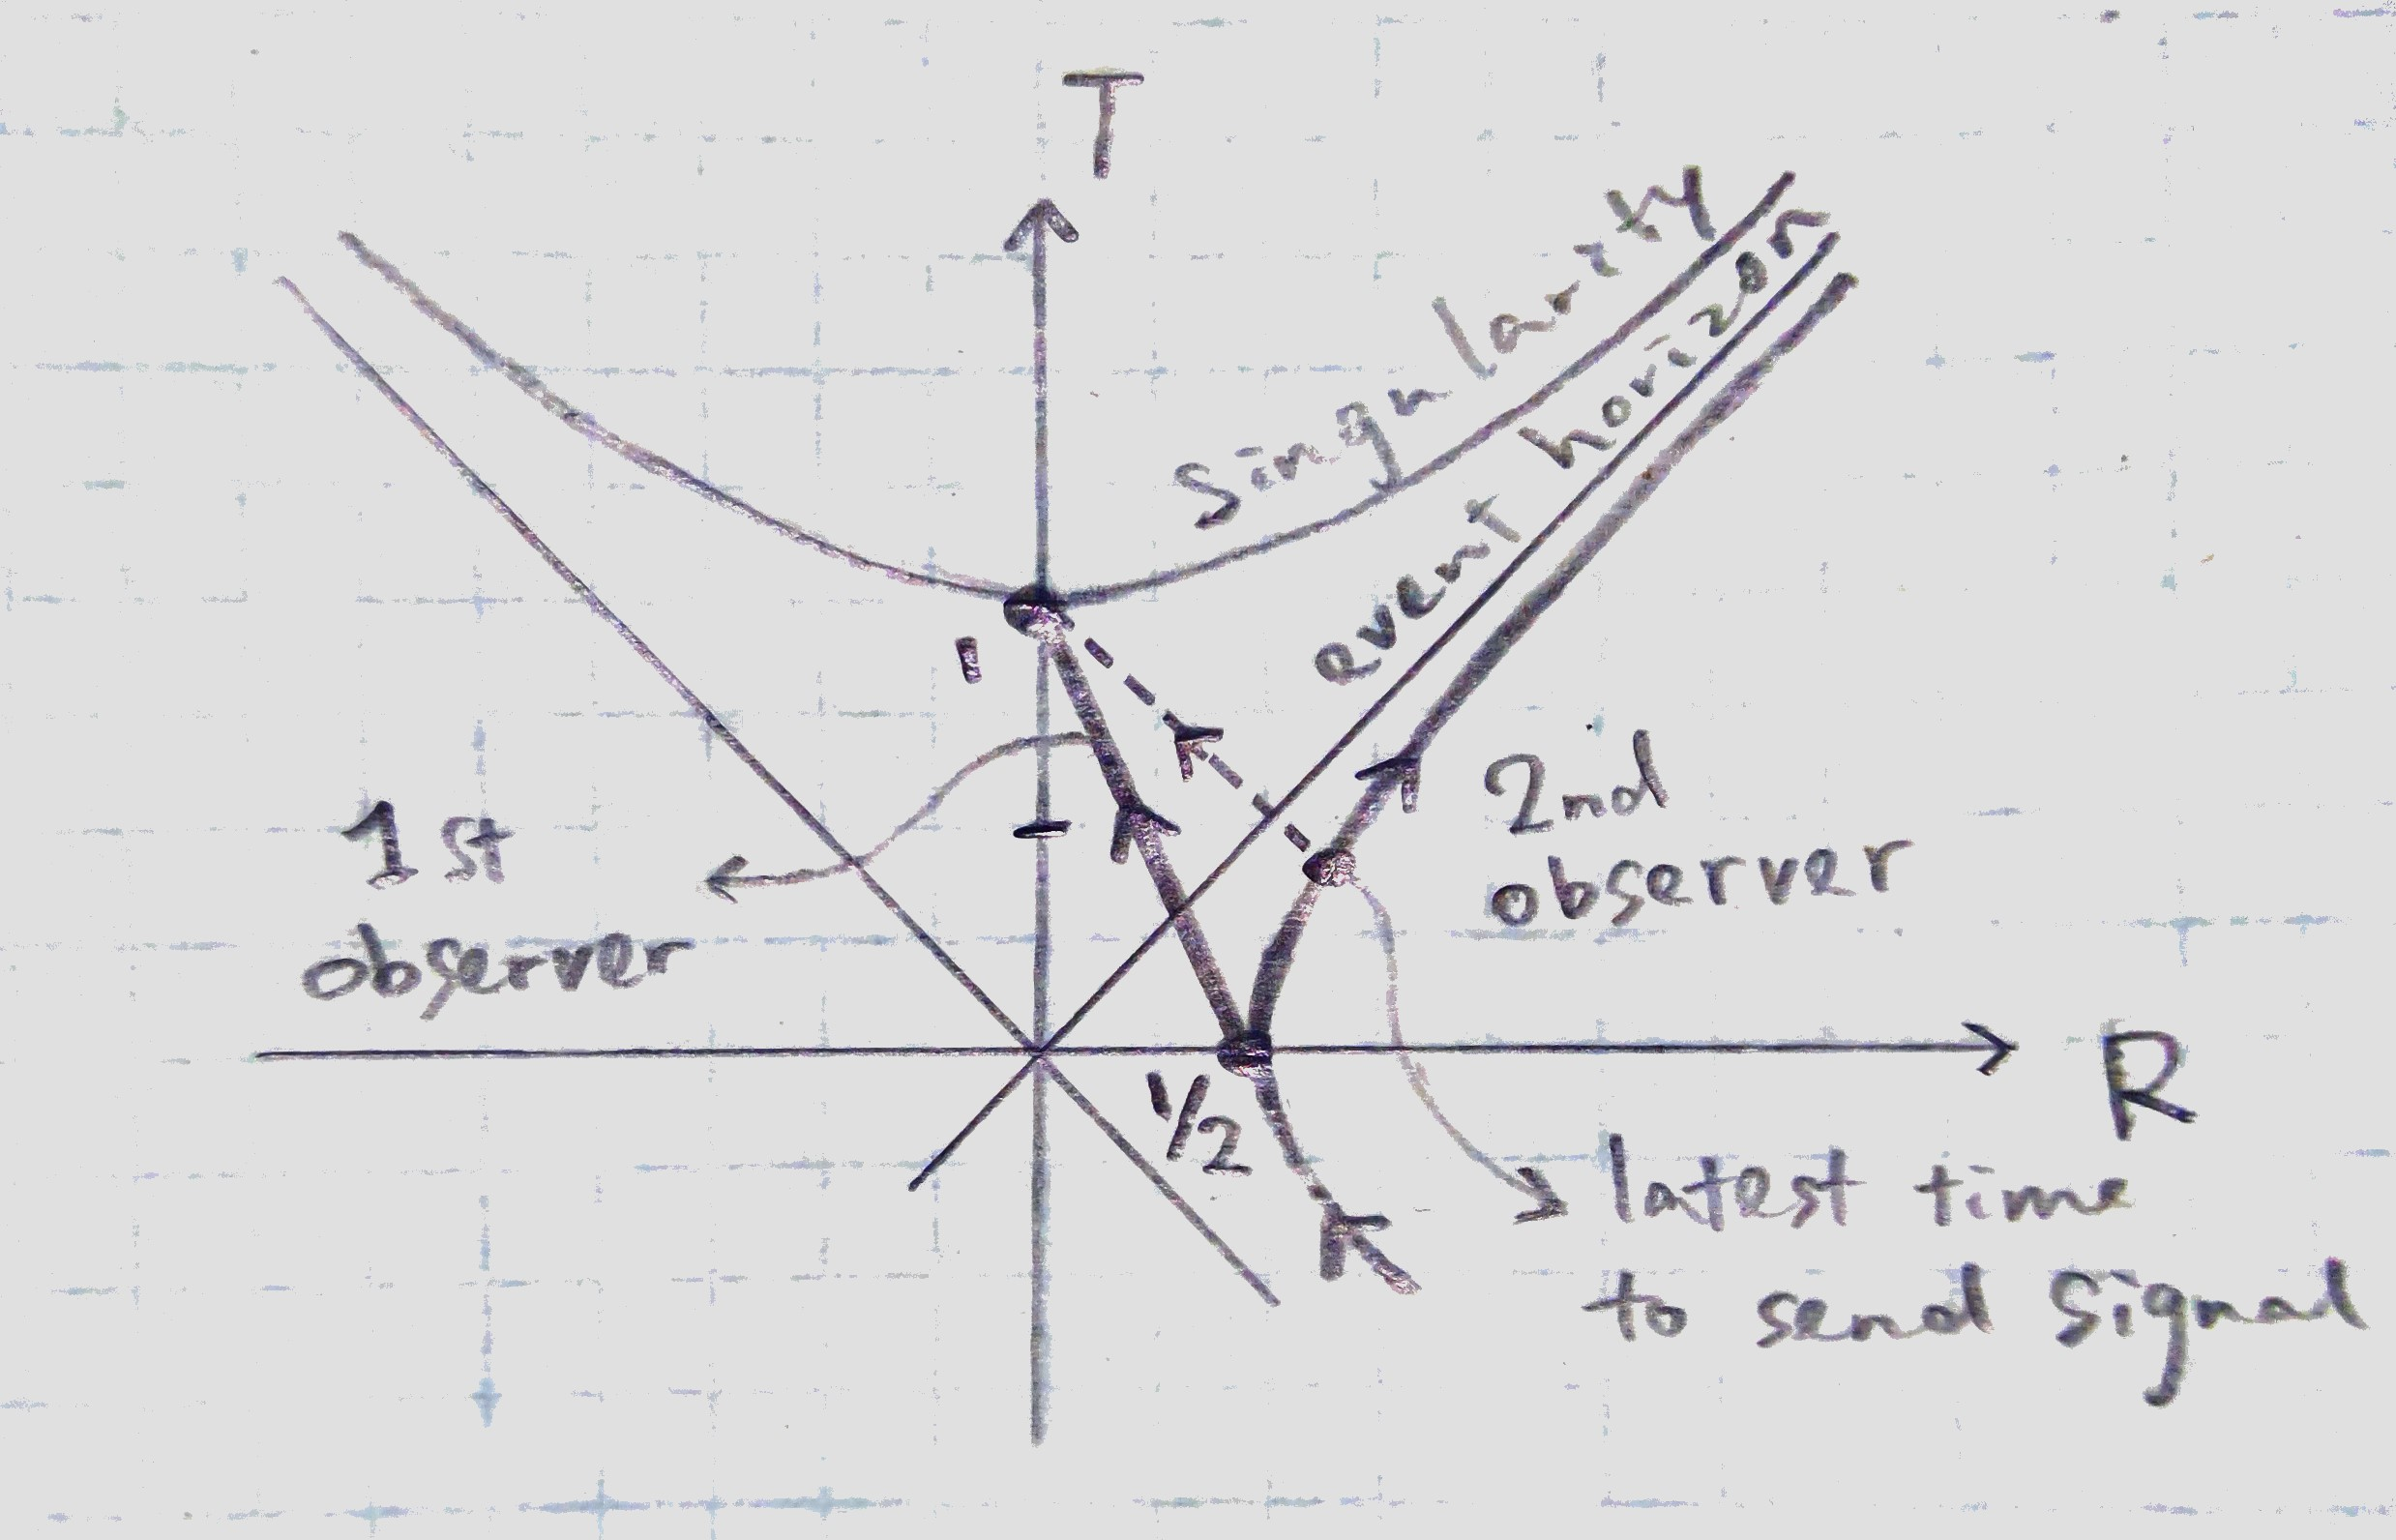
\includegraphics[width=0.8\textwidth]{diagram-1.jpg}
\end{center}
\subsection*{b}
Yes, because the worldline lies within the $45^\circ$ light cone at each point.
\subsection*{c}
For the second observer at constant $r$,
\[  T = \frac{1}{2}\sinh\left( \frac{t}{4GM} \right), \quad R = \frac{1}{2}\cosh\left( \frac{t}{4GM} \right)
	,\quad R^2 - T^2 = \frac{1}{4} \]
To reach the critical point where the first observer is destroyed, the photon sent by the second observer must follow the straight line $R  = 1 - T$, which intersects the second observer's worldline in the past at
\[ \cancel{T^2} - 2T + 1 - \cancel{T^2} = \frac{1}{4} \Rightarrow\quad T = \frac{1}{2}\sinh\left( \frac{t}{4GM} \right)  = \frac{3}{8}\]
\[ t = 4GM\sinh^{-1}\left(\frac{3}{4}\right) \approx 2.77GM \]
\section{}
A perfect fluid is incompressible, therefore $\nabla_\mu \rho = \partial_\mu \rho = 0$. From the continuity equation,
\[ \nabla_\mu(\rho u^\mu) =  \rho \nabla_\mu u^\mu = 0 \quad\Rightarrow\quad \nabla_\mu u^\mu = 0\]
The conservation law requires the covariant divergence of stress-energy tensor to vanish:
\begin{align*}
\nabla_\mu T^\mu{}_\nu &= (\nabla_\mu p + \cancel{\nabla_\mu\rho}) u^\mu u_\nu + (p+\rho) \cancel{(\nabla_\mu u^\mu)} u_\nu + (p+\rho) u^\mu (\nabla_\mu u_\nu) + \delta^\mu_\nu \nabla_\mu p \\
&= u_\nu (u^\mu \nabla_\mu p)  + (p+\rho) (u^\mu \nabla_\mu u_\nu) + (\delta^\mu_\nu \nabla_\mu) p \\
&=  u_\nu \nabla_{\ut{u}} p  + (p+\rho) \nabla_{\ut{u}} u_\nu + \nabla_\nu p  \\
&= 0
\end{align*}
Rearranging the terms (and dropping the free index $\nu$) gives
\[ (p + \rho)\nabla_{\ut{u}}\ut{u} = - \nabla p - \ut{u}\nabla_{\ut{u}}p \]

\end{document}